\section{Performance Validation in Simulation - (Lead by Abhishek, Amelia, Lucian, Vlad)}\label{sec:mc}

% The charge collection of the MALTA2 pixel has been derived from testbeam data \cite{MALTA2_CCParameterization}.
% A parametric simulation approach is used that has been validated against data \cite{FastSim}.
As discussd in section (ref section 3.1) and shoen in Fig.2 (ref fig2) a quad module made of four MALTA2 sensors in series is simulated in GEANT4.
Each sensor is identical and placed horizontally adjacent to each other, as shown in Fig.~\ref{fig:geom}.
Each MALTA2 sensor is implemented in a data-driven fast simulation method. 
A detailed characterization and implementation of this fast simulation approach is described in Ref.~\cite{FastSim}.
This study primararily focuses on the abilty of reconstruction of signals (pions) by the MALTA2 sensors in the presence of background particles, 
mostly electrons and positrons, that are expected to be present near the beam-pipe of EIC. A detailed studey of the background rate and 
its impact on the performance of the MALTA2 sensors is presented in the following subsections.

\subsection{Telescope geometry and setup in simulation}\label{sec:geometry}
Each quad module consists of four MALTA2 sensors placed side by side in the $xy$ plane as shown in Fig.~\ref{fig:geom} with
negligible gap of $ \approx$1$\mu m$. 
The sensor positions are listed in Table~\ref{tab:geom}. A 29 $\mu m$ thick silicon layer is used to construct sensor and 
it is defined as senstive detector volume in GEANT4. Both Elecromagnetism and Hadronic physics list are being used her to used in
this simulation. We used GEANT4 particle gun to generate signal particles in a longitudinal direction
and it is centered at (18.64, 0.0, -1000.0) mm.
\begin{equation}
    D^{0} \rightarrow K^{-} \pi^{+}, \qquad \bar{D}^{0} \rightarrow K^{+} \pi^{-}.
    \label{eq:d0decay}
\end{equation}
Positive charged Pions are used as our signal particles since they are decay-products of $D^{0}$ as shown in Eq.~\ref{eq:d0decay}.
Signal-beam particles are generated from a three-dimensional Gaussian distribution, with standard deviations of 0.5~mm in $x$ and $y$ and 100~mm in $z$.
The generated vertex distribution is shown in Fig.~\ref{fig:genXYZ}. These particles deposits energy in the sensor and 
the charge collection is simulated using the data-driven fast simulation method described in Ref.~\cite{FastSim}. Along with
charge collection, a paramteric model for time-walk is used here to simulate realistic MALTA2 sensor timing ans it is explained 
in Ref.~\cite{FastSim}.
The two-dimensional distribution of raw hits is shown in Fig.~\ref{fig:rawhits2D}. After that this 
charge is digitized and the hit information is stored in a ROOT file for further analysis. 
Signal beam has a veto of \SI{2}{\micro\second} (cite Xuan arxiv paper \href{https://arxiv.org/html/2410.00837v1})
and energy of 1 GeV and this is taken from the fact that EIC has bunch-crossing of 10.2 ns but signal only produces every \SI{2}{\micro\second}.
These signal particles are reconstructed by the sensors in both planes and those hits are matched with generated truth tracks both spatially
and temporarily window. If a Hit (X,Y) on sensor is with in radius of 100 $\mu$m and within 500 $ns$ time window with refernce to generated truth. It will be matched with
generated truth and defined as Hit matching. We define a hit efficiency as the ratio of the number of signal particles that are reconstructed by the sensor to the total number of signal particles
generated in the simulation. Without any bcakground and signal hit efficiency for 1 GeV Pion is $\approx~96.8\%$. The efficiency here is 
lost in two component firsr major compnent is pion's short life-time. A 1 GeV Pion has probability of decay $\approx~1.6\%$. Second compoenent
is charge sharing among 4 pixels and a signal below threshold of 150 e- can be lost. If Pion life-time set infinite in simulation ist Hit
efficiency is $\approx~99\%$ for the plane 0.


\begin{figure}[H]
    \centering
    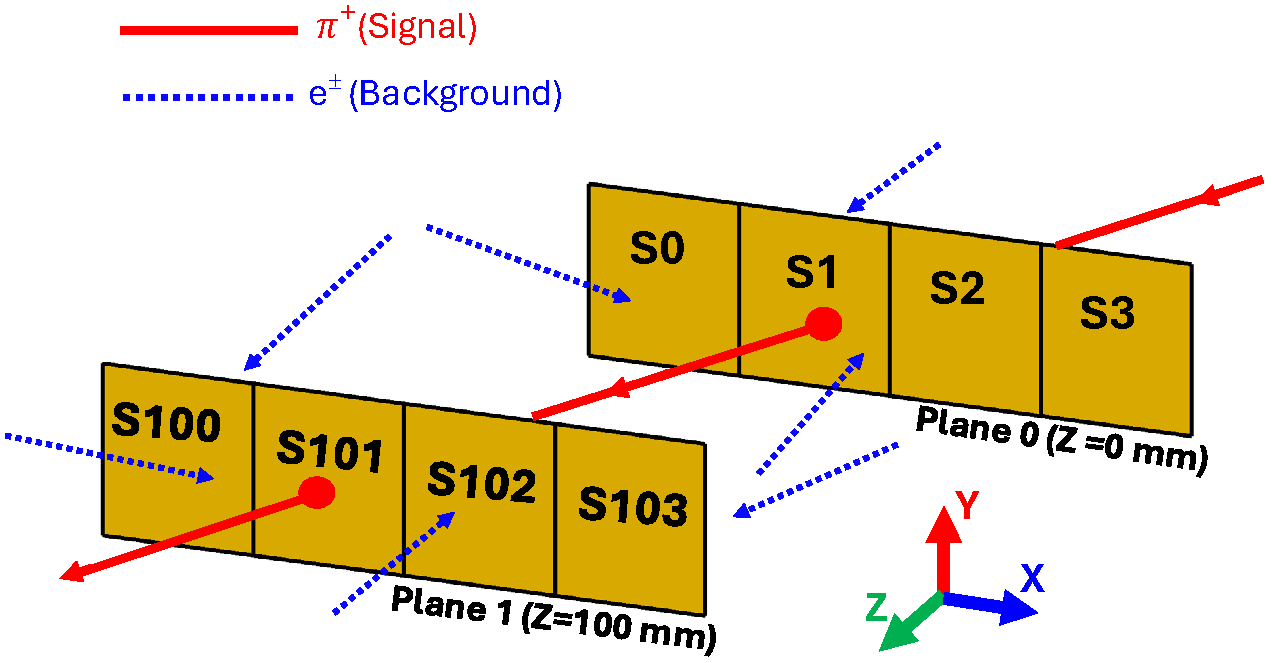
\includegraphics[width=0.5\textwidth]{Figures/geom.pdf}
    \caption{%
        MALTA QUAD Module geometry: eight $18.6 \times 18.6$~mm$^{2}$ silicon sensors in two planes separated by 100~mm.
        Red: \SI{1}{GeV} $\pi^{+}$ signal beam generated at $z = -1000$~mm and focused on the second sensor (S1 \& S101) of each plane.
        Blue dashed: randomly generated background $e^{-}/e^{+}$.
    }
    \label{fig:geom}
\end{figure}

\begin{table}[H]
    \centering
    \caption{%
        Positions of the eight MALTA2 sensors in the quad-module geometry.
        All sensors lie in the $y = 0$ plane and are placed side by side along $x$.
    }
    \label{tab:geom}
    \begin{tabular}{c c c c c c}
        \hline
        Plane & $z$ [mm] & \multicolumn{4}{c}{Sensor $x$-centre [mm]} \\
        & & S0 & S1 & S2 & S3 \\
        \hline
        0 & 0   & 0.00 & 18.64 & 37.27 & 55.91 \\
        1 & 100 & 0.00 & 18.64 & 37.27 & 55.91 \\
        \hline
    \end{tabular}
\end{table}

\begin{figure}[H]
    \centering
    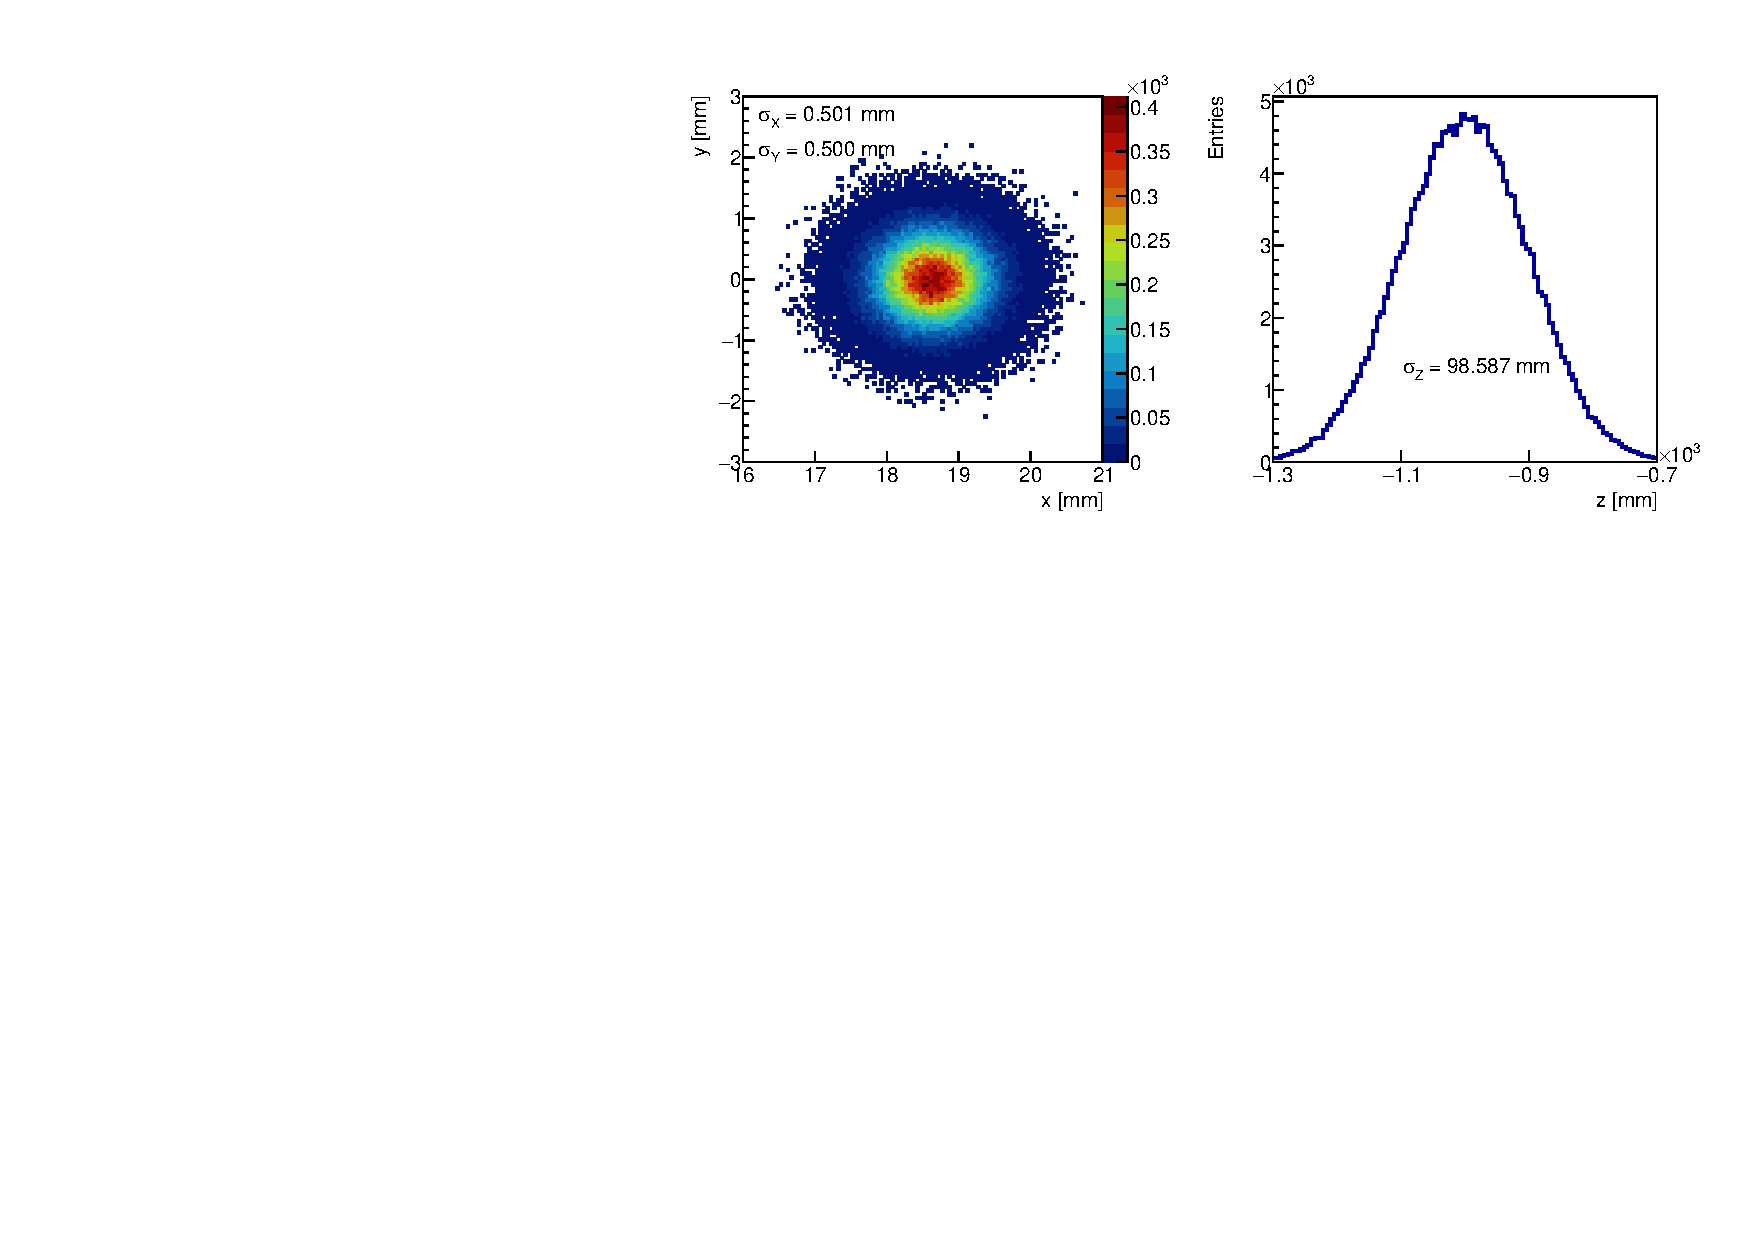
\includegraphics[width=\linewidth]{Figures/verify_gen_vertex.pdf}
    \caption{%
        Generated signal-beam vertex positions: (left) transverse $(x, y)$ distribution and (right) longitudinal $z$ distribution.
    }
    \label{fig:genXYZ}
\end{figure}


\begin{figure*}[t]
    \centering
    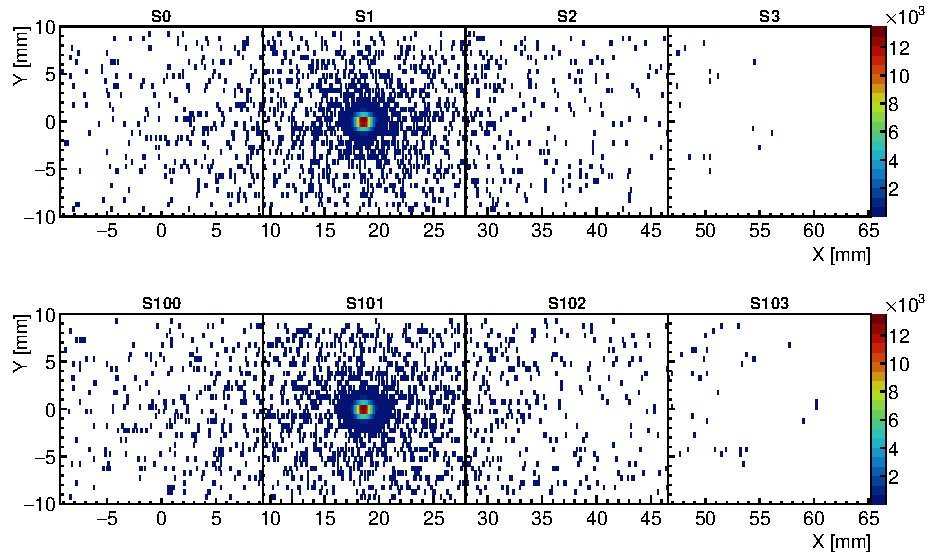
\includegraphics[width=\textwidth]{Figures/verify_2D_XY_both_planes.pdf}
    \caption{%
        Two-dimensional distribution of raw hits in the eight MALTA2 sensors.
        The top row shows sensors S0--S3 of the first plane (0) and the bottom row sensors S100--S103 of the second plane (1).
    }
    \label{fig:rawhits2D}
\end{figure*}

\subsection{Time Resolution (no background)}
\textcolor{red}{Plot: Time resolution (compare: without background, with 1,2,3 particles per event)}
Validated with data.

\subsection{Background rate}
Explain the expected background at the location of the FMT (from Amelia's plots?):
\begin{itemize}
    \item Select region of $1\times\SI{2}{\square\centi\meter}$ with highest hit rate.
    \item Show distribution of hits per $\SI{2}{\micro\second}$ event
    \item Show PDG code of background particles. Is it primarily photons and electrons/ positrons?
\end{itemize}

Explain the simplifications/ assumptions that go into the MALTA2 simulation.
\begin{itemize}
    \item Identify maximum expected background hit rate per sampled event.
    \item Spatial distribution is approximately flat within individual MALTA2 sensor.
\end{itemize}
To determine the expected background rate, projected plots were made using the EIC simulation files alongside PyROOT analysis. The EIC Geant4 simulation files used were the April 2026 FULL deep inelastic scattering neutral current background files. Since these were FULL files, each contained the Geant4 simulation ROOT files as well as truth level information. The Forward MPGD disk located at 1415 mm from the point of collision was used as a reference detector for the background environment near the proposed FMT location. By masking to the chosen z-location, it was possible to extract various background distributions at the disk location. In addition to the z-location “disk” mask, a “sensor” mask was applied to the disk as a way to isolate the footprint of one MALTA2 sensor within the disk. This “sensor” mask limited the x- and y- dimensions to that of one MALTA2 sensor with a final footprint of 1 by 2 cm\^2. 

To determine the peak background rate, the highest hit sensor was chosen out of several sensors near the beampipe. Because the hit and momentum distributions were of interest, the highest hit background sensor plots can be found in Fig. \ref{fig:expected_sensor_background} . The top left 2D histogram was used to determine the expected rate per event in the default 2 \(\mu s\) window by taking the integral of the plot. This resulted in an expected rate per event of 0.198. Additionally, this plot shows that the spatial distribution in this plot is relatively flat within an individual MALTA2 sensor.

Fig. \ref{fig:pdg_background} displays the PDG codes of the background hits at the Forward MPGD disk at z = 1415 mm. From this plot, it is clear that the primary background particles in this region are electrons (PDG = 11), positrons (PDG = -11), and photons (PDG = 22).

\begin{figure}
    \centering
    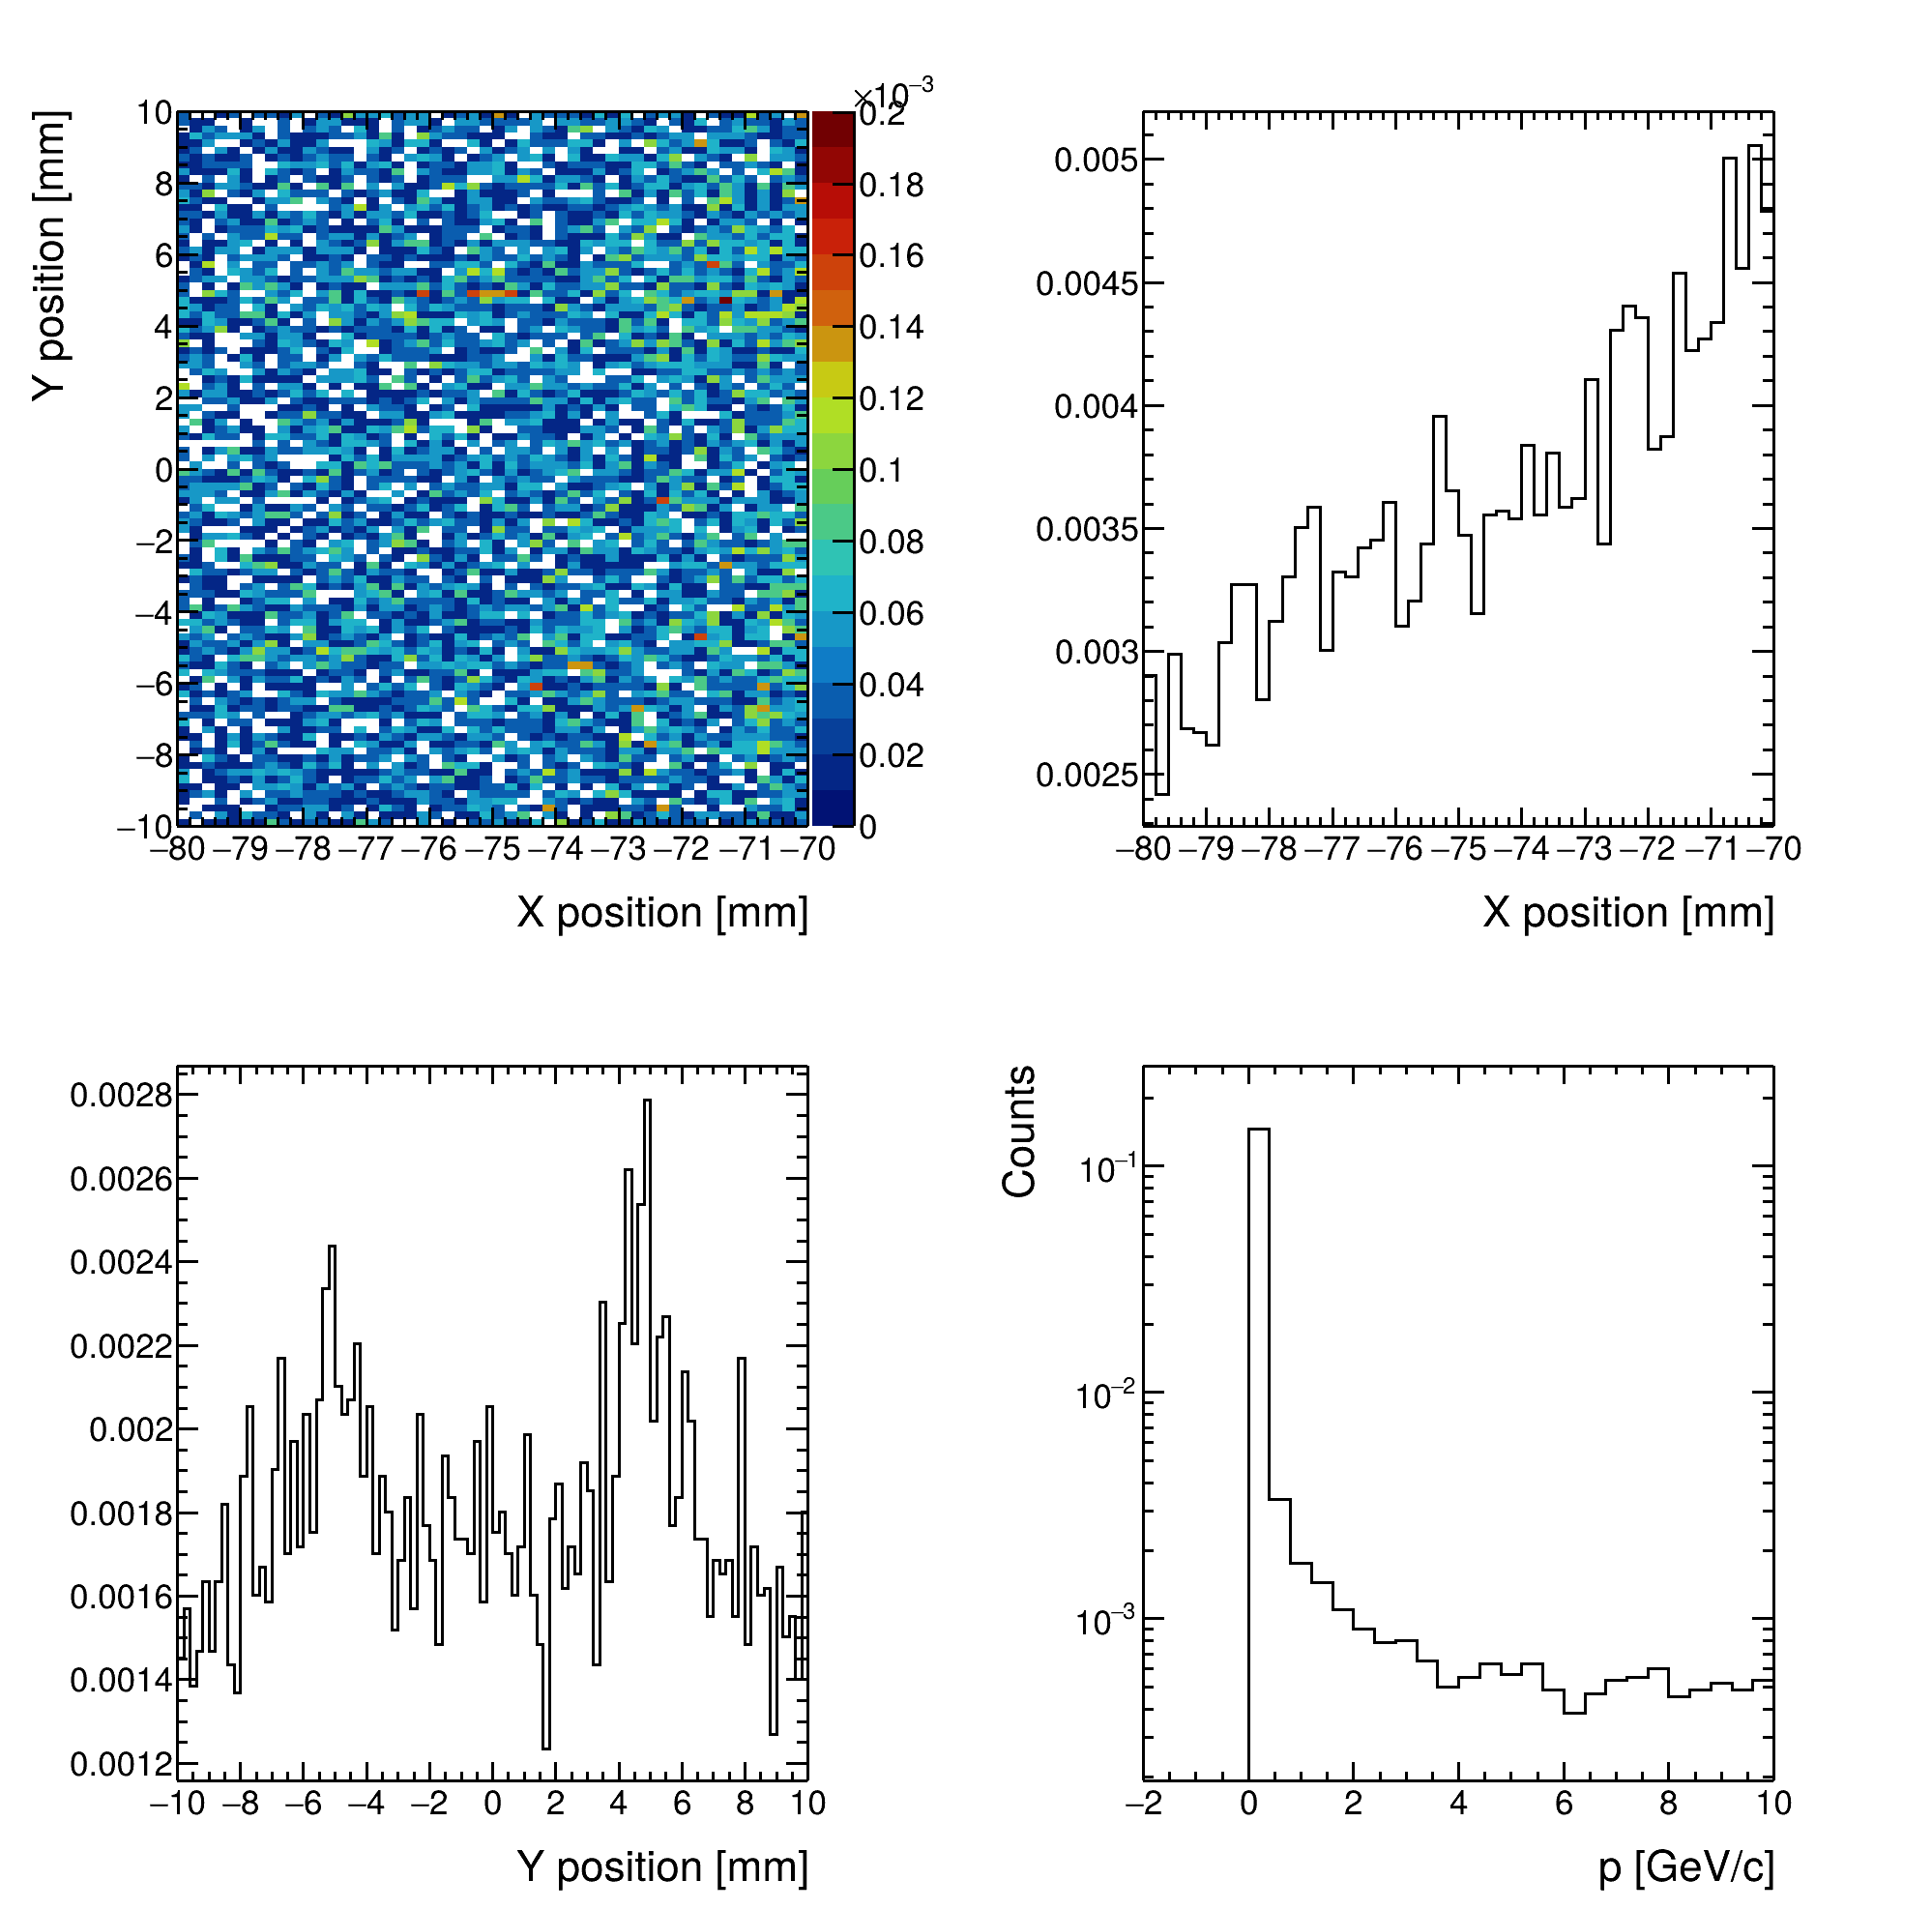
\includegraphics[width=0.75\linewidth]{Figures/EIC_current_background_AprilFULL.png}
    \caption{Expected background distributions for one MALTA2 sensor at 1415 mm from the collision point. Top left: 2D histogram of hits in the x- and y- dimensions; Top right: x-projection of hits; Bottom left: y-projection of hits; Bottom right: momentum magnitude distribution}
    \label{fig:expected_sensor_background}
\end{figure}
\begin{figure}
    \centering
    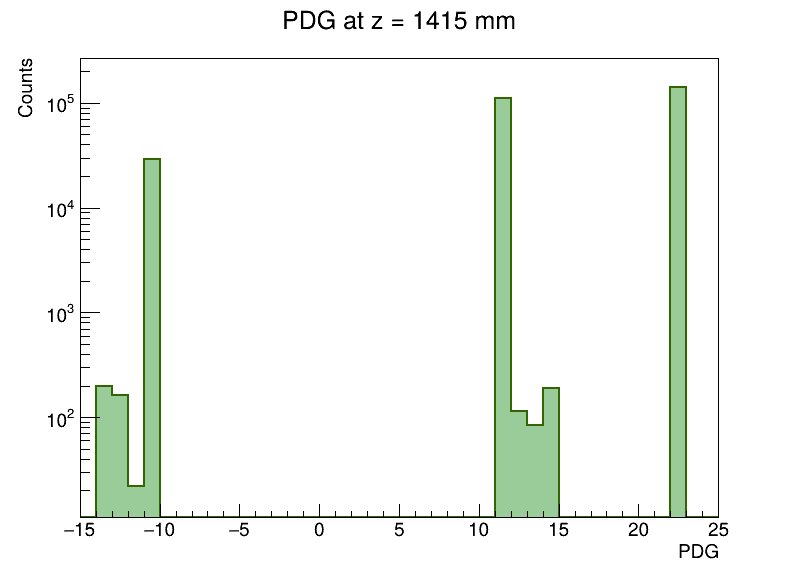
\includegraphics[width=0.5\linewidth]{Figures/MCParticles_1415_PDG_50files.png}
    \caption{Particle identification at reference detector Forward MPGD Disk z = 1415 mm. THIS PLOT NEEDS TO BE UPDATED TO FIT THE STYLE}
    \label{fig:pdg_background}
\end{figure}

\subsection{Sampling of EIC background}
The momentum magnitude distributions of the background electrons and positrons are each modelled by a Crystal Ball function.
The fitted parameters are used to sample the background momentum in every \SI{2}{\micro\second} window via inverse-transform sampling.
The corresponding fit for electrons is shown in Fig.~\ref{fig:bkgCB}.
Background vertices are generated uniformly within a three-dimensional box spanning the simulation world volume.
The direction of each background particle is chosen such that it always crosses one of the two detector planes, as shown in Fig.~\ref{fig:geom}.
After fixing momentum and random direction rate of background particle is sampled using poisson dstrubtuion. EIC background rate is 
$\approx~1.5$ particles per 2 $\mu$s. 


\begin{figure}[H]
    \centering
    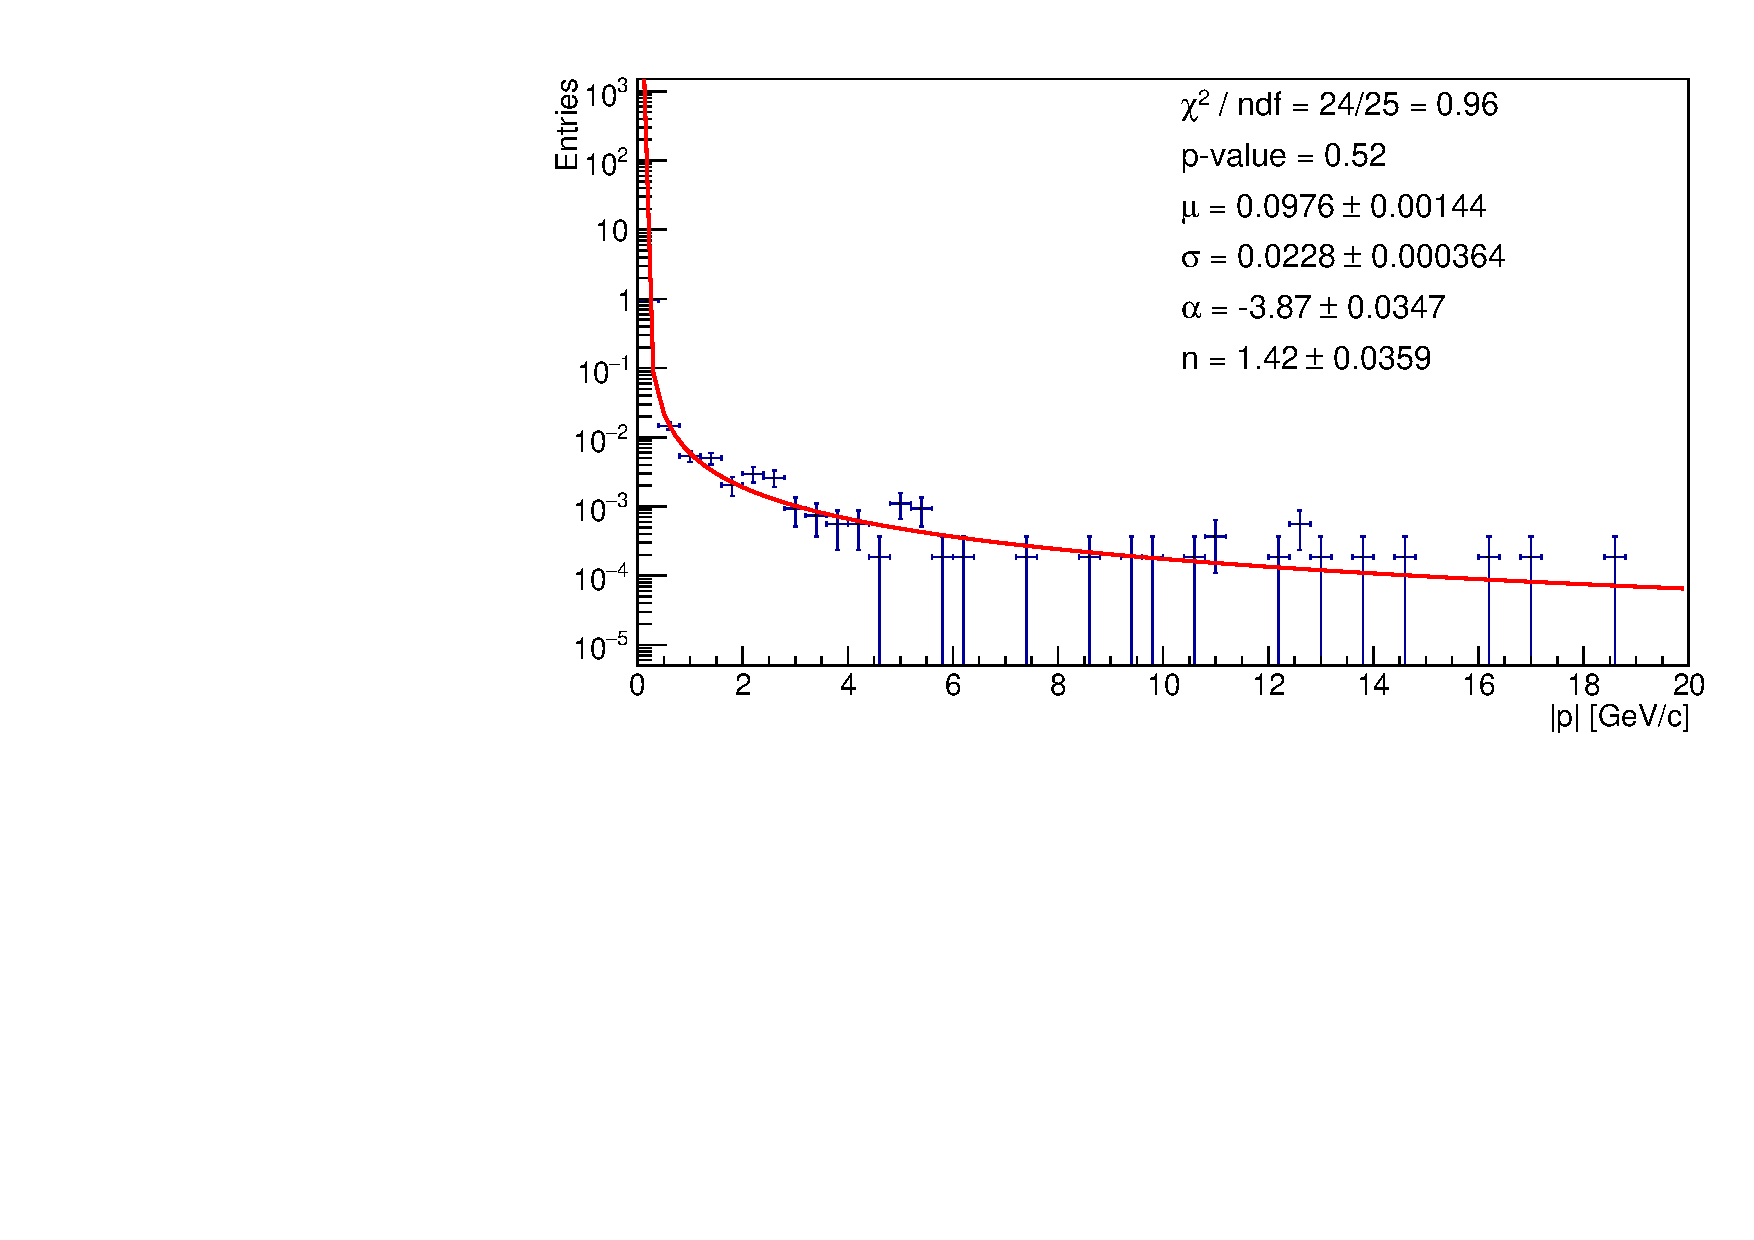
\includegraphics[width=\linewidth]{Figures/electron_cb_par_pmag.pdf}
    \caption{%
        Crystal Ball fit to the momentum magnitude distribution of background electrons.
    }
    \label{fig:bkgCB}
\end{figure}

\subsection{Hit efficiency with background}
The background rate is varied from zero to 15.84 particles per \SI{2}{\micro\second} event, and the hit efficiency is measured at each rate, as shown in Fig.~\ref{fig:bkgEff}.
The per-plane hit efficiency is defined as the fraction of signal pions that passed the Hit-matching critires defined in section~\ref{sec:geometry}
 in a given plane.
Plane 0 and plane 1 follow the same slow decrease with the background rate, with plane 1 systematically lower by about 1$\%$ because a fraction of the pions scattered between the two planes.
The coincidence efficiency requires a reconstructed hit in both planes within the coincidence window, and is therefore lower than either per-plane efficiency.
The coincidence efficiency decreases faster than the per-plane efficiencies because the signal pion is scattered in the first sensor layer, which displaces its 
hit position in the second plane and causes a small fraction of events to fail the coincidence requirement as the background occupancy increases.
In principle background particles are occupying the MALTA2 word-encoding 1.6 ns window and that hit becomes dispalced or changed- decrease 
in hit efficiency.

\begin{figure}[H]
    \centering
    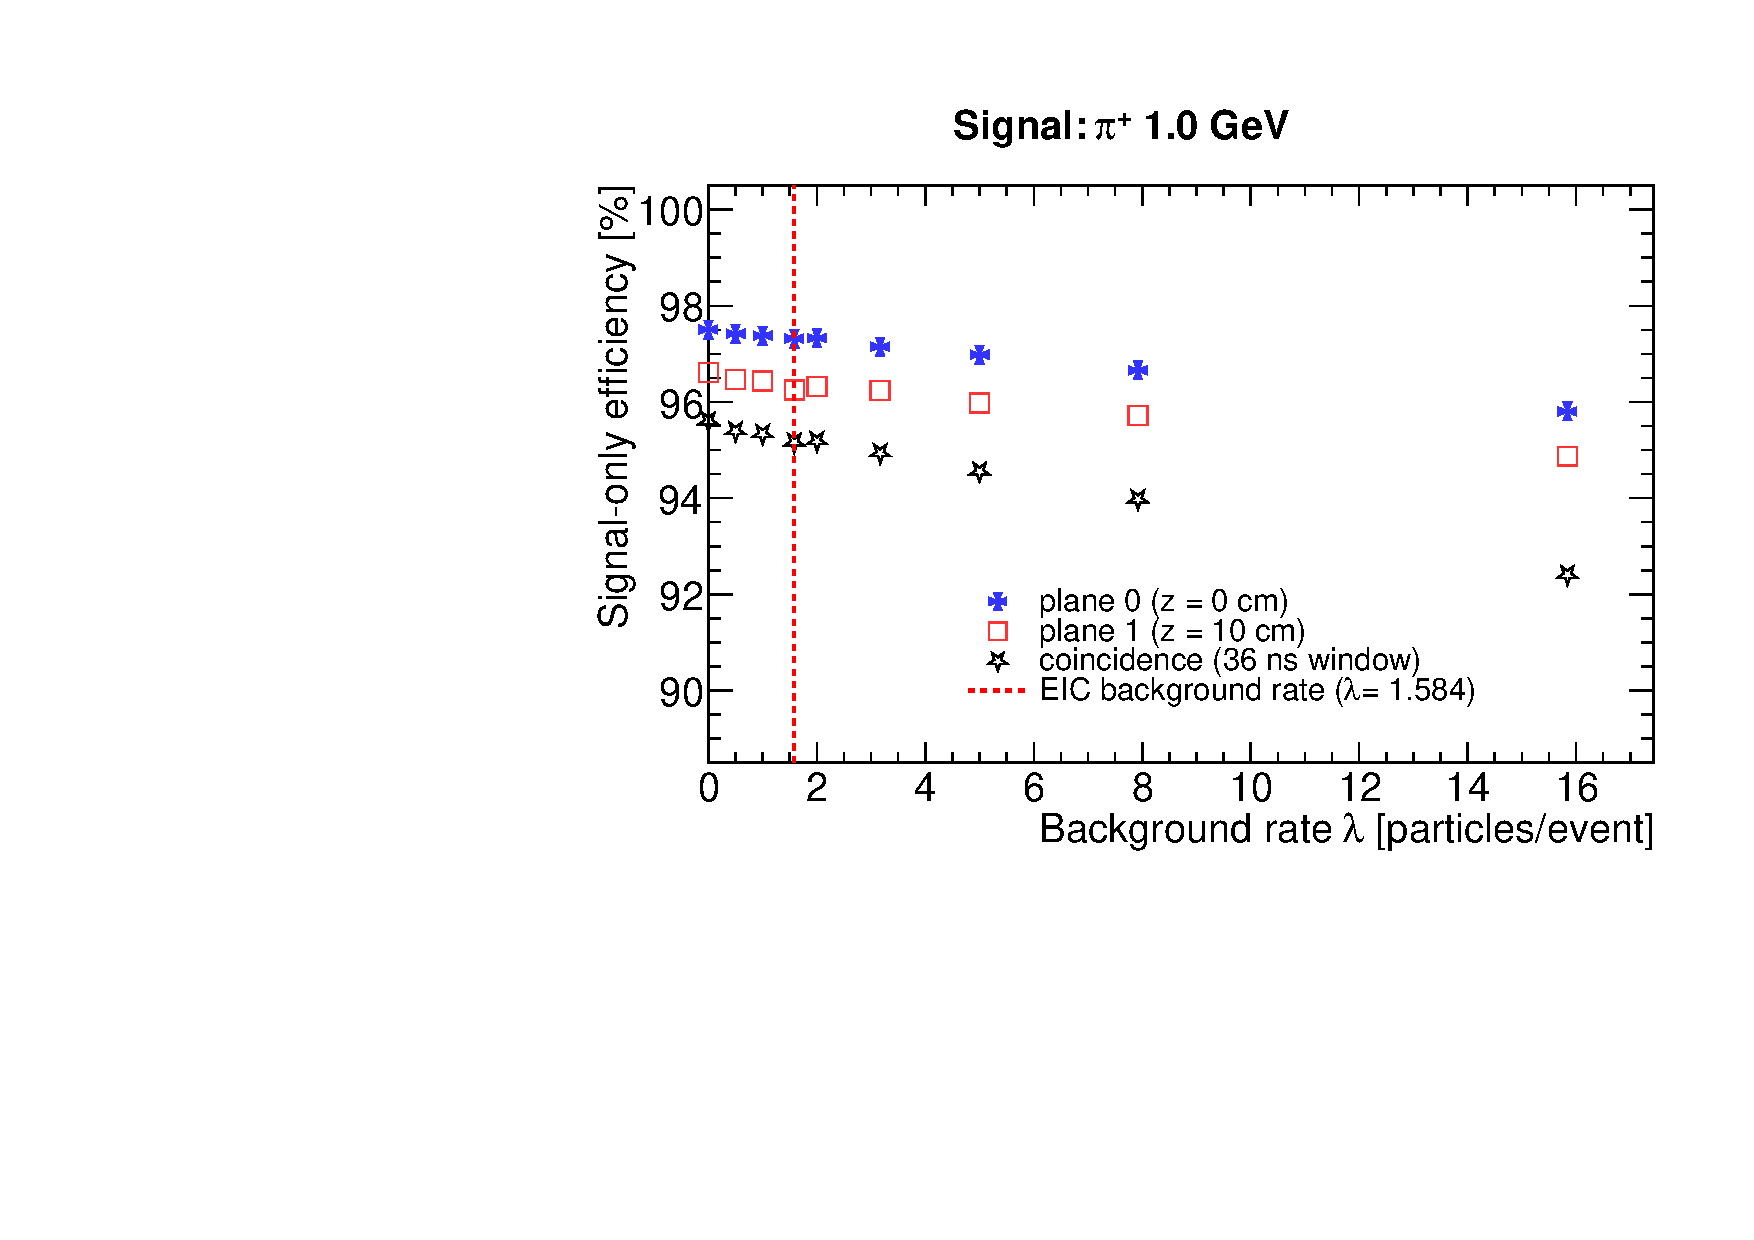
\includegraphics[width=\linewidth]{Figures/bkg_eff.pdf}
    \caption{%
        Hit efficiency as a function of the background rate for 1~GeV pions.
        Per-plane efficiencies are shown for plane 0 and plane 1, together with the coincidence efficiency.
    }
    \label{fig:bkgEff}
\end{figure}


\subsection{Tracking efficiency, potential spatial/temporal resolution with background}
This subsection can target the proper tracking efficiency using 2 FMT planes.
\begin{itemize}
    \item Obtain hits per plane.
    \item Reconstruct a track from the two planes.
    \item Calculate pointing resolution of the track. In the simulation, signal is incident perpendicular onto the sensor. How is the direction reconstructed from the track?
\end{itemize}

\subsection{Matching capability with background}
